
% Default to the notebook output style

    


% Inherit from the specified cell style.




    
\documentclass[11pt]{article}

    
    
    \usepackage[T1]{fontenc}
    % Nicer default font (+ math font) than Computer Modern for most use cases
    \usepackage{mathpazo}

    % Basic figure setup, for now with no caption control since it's done
    % automatically by Pandoc (which extracts ![](path) syntax from Markdown).
    \usepackage{graphicx}
    % We will generate all images so they have a width \maxwidth. This means
    % that they will get their normal width if they fit onto the page, but
    % are scaled down if they would overflow the margins.
    \makeatletter
    \def\maxwidth{\ifdim\Gin@nat@width>\linewidth\linewidth
    \else\Gin@nat@width\fi}
    \makeatother
    \let\Oldincludegraphics\includegraphics
    % Set max figure width to be 80% of text width, for now hardcoded.
    \renewcommand{\includegraphics}[1]{\Oldincludegraphics[width=.8\maxwidth]{#1}}
    % Ensure that by default, figures have no caption (until we provide a
    % proper Figure object with a Caption API and a way to capture that
    % in the conversion process - todo).
    \usepackage{caption}
    \DeclareCaptionLabelFormat{nolabel}{}
    \captionsetup{labelformat=nolabel}

    \usepackage{adjustbox} % Used to constrain images to a maximum size 
    \usepackage{xcolor} % Allow colors to be defined
    \usepackage{enumerate} % Needed for markdown enumerations to work
    \usepackage{geometry} % Used to adjust the document margins
    \usepackage{amsmath} % Equations
    \usepackage{amssymb} % Equations
    \usepackage{textcomp} % defines textquotesingle
    % Hack from http://tex.stackexchange.com/a/47451/13684:
    \AtBeginDocument{%
        \def\PYZsq{\textquotesingle}% Upright quotes in Pygmentized code
    }
    \usepackage{upquote} % Upright quotes for verbatim code
    \usepackage{eurosym} % defines \euro
    \usepackage[mathletters]{ucs} % Extended unicode (utf-8) support
    \usepackage[utf8x]{inputenc} % Allow utf-8 characters in the tex document
    \usepackage{fancyvrb} % verbatim replacement that allows latex
    \usepackage{grffile} % extends the file name processing of package graphics 
                         % to support a larger range 
    % The hyperref package gives us a pdf with properly built
    % internal navigation ('pdf bookmarks' for the table of contents,
    % internal cross-reference links, web links for URLs, etc.)
    \usepackage{hyperref}
    \usepackage{longtable} % longtable support required by pandoc >1.10
    \usepackage{booktabs}  % table support for pandoc > 1.12.2
    \usepackage[inline]{enumitem} % IRkernel/repr support (it uses the enumerate* environment)
    \usepackage[normalem]{ulem} % ulem is needed to support strikethroughs (\sout)
                                % normalem makes italics be italics, not underlines
    

    
    
    % Colors for the hyperref package
    \definecolor{urlcolor}{rgb}{0,.145,.698}
    \definecolor{linkcolor}{rgb}{.71,0.21,0.01}
    \definecolor{citecolor}{rgb}{.12,.54,.11}

    % ANSI colors
    \definecolor{ansi-black}{HTML}{3E424D}
    \definecolor{ansi-black-intense}{HTML}{282C36}
    \definecolor{ansi-red}{HTML}{E75C58}
    \definecolor{ansi-red-intense}{HTML}{B22B31}
    \definecolor{ansi-green}{HTML}{00A250}
    \definecolor{ansi-green-intense}{HTML}{007427}
    \definecolor{ansi-yellow}{HTML}{DDB62B}
    \definecolor{ansi-yellow-intense}{HTML}{B27D12}
    \definecolor{ansi-blue}{HTML}{208FFB}
    \definecolor{ansi-blue-intense}{HTML}{0065CA}
    \definecolor{ansi-magenta}{HTML}{D160C4}
    \definecolor{ansi-magenta-intense}{HTML}{A03196}
    \definecolor{ansi-cyan}{HTML}{60C6C8}
    \definecolor{ansi-cyan-intense}{HTML}{258F8F}
    \definecolor{ansi-white}{HTML}{C5C1B4}
    \definecolor{ansi-white-intense}{HTML}{A1A6B2}

    % commands and environments needed by pandoc snippets
    % extracted from the output of `pandoc -s`
    \providecommand{\tightlist}{%
      \setlength{\itemsep}{0pt}\setlength{\parskip}{0pt}}
    \DefineVerbatimEnvironment{Highlighting}{Verbatim}{commandchars=\\\{\}}
    % Add ',fontsize=\small' for more characters per line
    \newenvironment{Shaded}{}{}
    \newcommand{\KeywordTok}[1]{\textcolor[rgb]{0.00,0.44,0.13}{\textbf{{#1}}}}
    \newcommand{\DataTypeTok}[1]{\textcolor[rgb]{0.56,0.13,0.00}{{#1}}}
    \newcommand{\DecValTok}[1]{\textcolor[rgb]{0.25,0.63,0.44}{{#1}}}
    \newcommand{\BaseNTok}[1]{\textcolor[rgb]{0.25,0.63,0.44}{{#1}}}
    \newcommand{\FloatTok}[1]{\textcolor[rgb]{0.25,0.63,0.44}{{#1}}}
    \newcommand{\CharTok}[1]{\textcolor[rgb]{0.25,0.44,0.63}{{#1}}}
    \newcommand{\StringTok}[1]{\textcolor[rgb]{0.25,0.44,0.63}{{#1}}}
    \newcommand{\CommentTok}[1]{\textcolor[rgb]{0.38,0.63,0.69}{\textit{{#1}}}}
    \newcommand{\OtherTok}[1]{\textcolor[rgb]{0.00,0.44,0.13}{{#1}}}
    \newcommand{\AlertTok}[1]{\textcolor[rgb]{1.00,0.00,0.00}{\textbf{{#1}}}}
    \newcommand{\FunctionTok}[1]{\textcolor[rgb]{0.02,0.16,0.49}{{#1}}}
    \newcommand{\RegionMarkerTok}[1]{{#1}}
    \newcommand{\ErrorTok}[1]{\textcolor[rgb]{1.00,0.00,0.00}{\textbf{{#1}}}}
    \newcommand{\NormalTok}[1]{{#1}}
    
    % Additional commands for more recent versions of Pandoc
    \newcommand{\ConstantTok}[1]{\textcolor[rgb]{0.53,0.00,0.00}{{#1}}}
    \newcommand{\SpecialCharTok}[1]{\textcolor[rgb]{0.25,0.44,0.63}{{#1}}}
    \newcommand{\VerbatimStringTok}[1]{\textcolor[rgb]{0.25,0.44,0.63}{{#1}}}
    \newcommand{\SpecialStringTok}[1]{\textcolor[rgb]{0.73,0.40,0.53}{{#1}}}
    \newcommand{\ImportTok}[1]{{#1}}
    \newcommand{\DocumentationTok}[1]{\textcolor[rgb]{0.73,0.13,0.13}{\textit{{#1}}}}
    \newcommand{\AnnotationTok}[1]{\textcolor[rgb]{0.38,0.63,0.69}{\textbf{\textit{{#1}}}}}
    \newcommand{\CommentVarTok}[1]{\textcolor[rgb]{0.38,0.63,0.69}{\textbf{\textit{{#1}}}}}
    \newcommand{\VariableTok}[1]{\textcolor[rgb]{0.10,0.09,0.49}{{#1}}}
    \newcommand{\ControlFlowTok}[1]{\textcolor[rgb]{0.00,0.44,0.13}{\textbf{{#1}}}}
    \newcommand{\OperatorTok}[1]{\textcolor[rgb]{0.40,0.40,0.40}{{#1}}}
    \newcommand{\BuiltInTok}[1]{{#1}}
    \newcommand{\ExtensionTok}[1]{{#1}}
    \newcommand{\PreprocessorTok}[1]{\textcolor[rgb]{0.74,0.48,0.00}{{#1}}}
    \newcommand{\AttributeTok}[1]{\textcolor[rgb]{0.49,0.56,0.16}{{#1}}}
    \newcommand{\InformationTok}[1]{\textcolor[rgb]{0.38,0.63,0.69}{\textbf{\textit{{#1}}}}}
    \newcommand{\WarningTok}[1]{\textcolor[rgb]{0.38,0.63,0.69}{\textbf{\textit{{#1}}}}}
    
    
    % Define a nice break command that doesn't care if a line doesn't already
    % exist.
    \def\br{\hspace*{\fill} \\* }
    % Math Jax compatability definitions
    \def\gt{>}
    \def\lt{<}
    % Document parameters
    \title{tensorflow\_tutorial}
    
    
    

    % Pygments definitions
    
\makeatletter
\def\PY@reset{\let\PY@it=\relax \let\PY@bf=\relax%
    \let\PY@ul=\relax \let\PY@tc=\relax%
    \let\PY@bc=\relax \let\PY@ff=\relax}
\def\PY@tok#1{\csname PY@tok@#1\endcsname}
\def\PY@toks#1+{\ifx\relax#1\empty\else%
    \PY@tok{#1}\expandafter\PY@toks\fi}
\def\PY@do#1{\PY@bc{\PY@tc{\PY@ul{%
    \PY@it{\PY@bf{\PY@ff{#1}}}}}}}
\def\PY#1#2{\PY@reset\PY@toks#1+\relax+\PY@do{#2}}

\expandafter\def\csname PY@tok@w\endcsname{\def\PY@tc##1{\textcolor[rgb]{0.73,0.73,0.73}{##1}}}
\expandafter\def\csname PY@tok@c\endcsname{\let\PY@it=\textit\def\PY@tc##1{\textcolor[rgb]{0.25,0.50,0.50}{##1}}}
\expandafter\def\csname PY@tok@cp\endcsname{\def\PY@tc##1{\textcolor[rgb]{0.74,0.48,0.00}{##1}}}
\expandafter\def\csname PY@tok@k\endcsname{\let\PY@bf=\textbf\def\PY@tc##1{\textcolor[rgb]{0.00,0.50,0.00}{##1}}}
\expandafter\def\csname PY@tok@kp\endcsname{\def\PY@tc##1{\textcolor[rgb]{0.00,0.50,0.00}{##1}}}
\expandafter\def\csname PY@tok@kt\endcsname{\def\PY@tc##1{\textcolor[rgb]{0.69,0.00,0.25}{##1}}}
\expandafter\def\csname PY@tok@o\endcsname{\def\PY@tc##1{\textcolor[rgb]{0.40,0.40,0.40}{##1}}}
\expandafter\def\csname PY@tok@ow\endcsname{\let\PY@bf=\textbf\def\PY@tc##1{\textcolor[rgb]{0.67,0.13,1.00}{##1}}}
\expandafter\def\csname PY@tok@nb\endcsname{\def\PY@tc##1{\textcolor[rgb]{0.00,0.50,0.00}{##1}}}
\expandafter\def\csname PY@tok@nf\endcsname{\def\PY@tc##1{\textcolor[rgb]{0.00,0.00,1.00}{##1}}}
\expandafter\def\csname PY@tok@nc\endcsname{\let\PY@bf=\textbf\def\PY@tc##1{\textcolor[rgb]{0.00,0.00,1.00}{##1}}}
\expandafter\def\csname PY@tok@nn\endcsname{\let\PY@bf=\textbf\def\PY@tc##1{\textcolor[rgb]{0.00,0.00,1.00}{##1}}}
\expandafter\def\csname PY@tok@ne\endcsname{\let\PY@bf=\textbf\def\PY@tc##1{\textcolor[rgb]{0.82,0.25,0.23}{##1}}}
\expandafter\def\csname PY@tok@nv\endcsname{\def\PY@tc##1{\textcolor[rgb]{0.10,0.09,0.49}{##1}}}
\expandafter\def\csname PY@tok@no\endcsname{\def\PY@tc##1{\textcolor[rgb]{0.53,0.00,0.00}{##1}}}
\expandafter\def\csname PY@tok@nl\endcsname{\def\PY@tc##1{\textcolor[rgb]{0.63,0.63,0.00}{##1}}}
\expandafter\def\csname PY@tok@ni\endcsname{\let\PY@bf=\textbf\def\PY@tc##1{\textcolor[rgb]{0.60,0.60,0.60}{##1}}}
\expandafter\def\csname PY@tok@na\endcsname{\def\PY@tc##1{\textcolor[rgb]{0.49,0.56,0.16}{##1}}}
\expandafter\def\csname PY@tok@nt\endcsname{\let\PY@bf=\textbf\def\PY@tc##1{\textcolor[rgb]{0.00,0.50,0.00}{##1}}}
\expandafter\def\csname PY@tok@nd\endcsname{\def\PY@tc##1{\textcolor[rgb]{0.67,0.13,1.00}{##1}}}
\expandafter\def\csname PY@tok@s\endcsname{\def\PY@tc##1{\textcolor[rgb]{0.73,0.13,0.13}{##1}}}
\expandafter\def\csname PY@tok@sd\endcsname{\let\PY@it=\textit\def\PY@tc##1{\textcolor[rgb]{0.73,0.13,0.13}{##1}}}
\expandafter\def\csname PY@tok@si\endcsname{\let\PY@bf=\textbf\def\PY@tc##1{\textcolor[rgb]{0.73,0.40,0.53}{##1}}}
\expandafter\def\csname PY@tok@se\endcsname{\let\PY@bf=\textbf\def\PY@tc##1{\textcolor[rgb]{0.73,0.40,0.13}{##1}}}
\expandafter\def\csname PY@tok@sr\endcsname{\def\PY@tc##1{\textcolor[rgb]{0.73,0.40,0.53}{##1}}}
\expandafter\def\csname PY@tok@ss\endcsname{\def\PY@tc##1{\textcolor[rgb]{0.10,0.09,0.49}{##1}}}
\expandafter\def\csname PY@tok@sx\endcsname{\def\PY@tc##1{\textcolor[rgb]{0.00,0.50,0.00}{##1}}}
\expandafter\def\csname PY@tok@m\endcsname{\def\PY@tc##1{\textcolor[rgb]{0.40,0.40,0.40}{##1}}}
\expandafter\def\csname PY@tok@gh\endcsname{\let\PY@bf=\textbf\def\PY@tc##1{\textcolor[rgb]{0.00,0.00,0.50}{##1}}}
\expandafter\def\csname PY@tok@gu\endcsname{\let\PY@bf=\textbf\def\PY@tc##1{\textcolor[rgb]{0.50,0.00,0.50}{##1}}}
\expandafter\def\csname PY@tok@gd\endcsname{\def\PY@tc##1{\textcolor[rgb]{0.63,0.00,0.00}{##1}}}
\expandafter\def\csname PY@tok@gi\endcsname{\def\PY@tc##1{\textcolor[rgb]{0.00,0.63,0.00}{##1}}}
\expandafter\def\csname PY@tok@gr\endcsname{\def\PY@tc##1{\textcolor[rgb]{1.00,0.00,0.00}{##1}}}
\expandafter\def\csname PY@tok@ge\endcsname{\let\PY@it=\textit}
\expandafter\def\csname PY@tok@gs\endcsname{\let\PY@bf=\textbf}
\expandafter\def\csname PY@tok@gp\endcsname{\let\PY@bf=\textbf\def\PY@tc##1{\textcolor[rgb]{0.00,0.00,0.50}{##1}}}
\expandafter\def\csname PY@tok@go\endcsname{\def\PY@tc##1{\textcolor[rgb]{0.53,0.53,0.53}{##1}}}
\expandafter\def\csname PY@tok@gt\endcsname{\def\PY@tc##1{\textcolor[rgb]{0.00,0.27,0.87}{##1}}}
\expandafter\def\csname PY@tok@err\endcsname{\def\PY@bc##1{\setlength{\fboxsep}{0pt}\fcolorbox[rgb]{1.00,0.00,0.00}{1,1,1}{\strut ##1}}}
\expandafter\def\csname PY@tok@kc\endcsname{\let\PY@bf=\textbf\def\PY@tc##1{\textcolor[rgb]{0.00,0.50,0.00}{##1}}}
\expandafter\def\csname PY@tok@kd\endcsname{\let\PY@bf=\textbf\def\PY@tc##1{\textcolor[rgb]{0.00,0.50,0.00}{##1}}}
\expandafter\def\csname PY@tok@kn\endcsname{\let\PY@bf=\textbf\def\PY@tc##1{\textcolor[rgb]{0.00,0.50,0.00}{##1}}}
\expandafter\def\csname PY@tok@kr\endcsname{\let\PY@bf=\textbf\def\PY@tc##1{\textcolor[rgb]{0.00,0.50,0.00}{##1}}}
\expandafter\def\csname PY@tok@bp\endcsname{\def\PY@tc##1{\textcolor[rgb]{0.00,0.50,0.00}{##1}}}
\expandafter\def\csname PY@tok@fm\endcsname{\def\PY@tc##1{\textcolor[rgb]{0.00,0.00,1.00}{##1}}}
\expandafter\def\csname PY@tok@vc\endcsname{\def\PY@tc##1{\textcolor[rgb]{0.10,0.09,0.49}{##1}}}
\expandafter\def\csname PY@tok@vg\endcsname{\def\PY@tc##1{\textcolor[rgb]{0.10,0.09,0.49}{##1}}}
\expandafter\def\csname PY@tok@vi\endcsname{\def\PY@tc##1{\textcolor[rgb]{0.10,0.09,0.49}{##1}}}
\expandafter\def\csname PY@tok@vm\endcsname{\def\PY@tc##1{\textcolor[rgb]{0.10,0.09,0.49}{##1}}}
\expandafter\def\csname PY@tok@sa\endcsname{\def\PY@tc##1{\textcolor[rgb]{0.73,0.13,0.13}{##1}}}
\expandafter\def\csname PY@tok@sb\endcsname{\def\PY@tc##1{\textcolor[rgb]{0.73,0.13,0.13}{##1}}}
\expandafter\def\csname PY@tok@sc\endcsname{\def\PY@tc##1{\textcolor[rgb]{0.73,0.13,0.13}{##1}}}
\expandafter\def\csname PY@tok@dl\endcsname{\def\PY@tc##1{\textcolor[rgb]{0.73,0.13,0.13}{##1}}}
\expandafter\def\csname PY@tok@s2\endcsname{\def\PY@tc##1{\textcolor[rgb]{0.73,0.13,0.13}{##1}}}
\expandafter\def\csname PY@tok@sh\endcsname{\def\PY@tc##1{\textcolor[rgb]{0.73,0.13,0.13}{##1}}}
\expandafter\def\csname PY@tok@s1\endcsname{\def\PY@tc##1{\textcolor[rgb]{0.73,0.13,0.13}{##1}}}
\expandafter\def\csname PY@tok@mb\endcsname{\def\PY@tc##1{\textcolor[rgb]{0.40,0.40,0.40}{##1}}}
\expandafter\def\csname PY@tok@mf\endcsname{\def\PY@tc##1{\textcolor[rgb]{0.40,0.40,0.40}{##1}}}
\expandafter\def\csname PY@tok@mh\endcsname{\def\PY@tc##1{\textcolor[rgb]{0.40,0.40,0.40}{##1}}}
\expandafter\def\csname PY@tok@mi\endcsname{\def\PY@tc##1{\textcolor[rgb]{0.40,0.40,0.40}{##1}}}
\expandafter\def\csname PY@tok@il\endcsname{\def\PY@tc##1{\textcolor[rgb]{0.40,0.40,0.40}{##1}}}
\expandafter\def\csname PY@tok@mo\endcsname{\def\PY@tc##1{\textcolor[rgb]{0.40,0.40,0.40}{##1}}}
\expandafter\def\csname PY@tok@ch\endcsname{\let\PY@it=\textit\def\PY@tc##1{\textcolor[rgb]{0.25,0.50,0.50}{##1}}}
\expandafter\def\csname PY@tok@cm\endcsname{\let\PY@it=\textit\def\PY@tc##1{\textcolor[rgb]{0.25,0.50,0.50}{##1}}}
\expandafter\def\csname PY@tok@cpf\endcsname{\let\PY@it=\textit\def\PY@tc##1{\textcolor[rgb]{0.25,0.50,0.50}{##1}}}
\expandafter\def\csname PY@tok@c1\endcsname{\let\PY@it=\textit\def\PY@tc##1{\textcolor[rgb]{0.25,0.50,0.50}{##1}}}
\expandafter\def\csname PY@tok@cs\endcsname{\let\PY@it=\textit\def\PY@tc##1{\textcolor[rgb]{0.25,0.50,0.50}{##1}}}

\def\PYZbs{\char`\\}
\def\PYZus{\char`\_}
\def\PYZob{\char`\{}
\def\PYZcb{\char`\}}
\def\PYZca{\char`\^}
\def\PYZam{\char`\&}
\def\PYZlt{\char`\<}
\def\PYZgt{\char`\>}
\def\PYZsh{\char`\#}
\def\PYZpc{\char`\%}
\def\PYZdl{\char`\$}
\def\PYZhy{\char`\-}
\def\PYZsq{\char`\'}
\def\PYZdq{\char`\"}
\def\PYZti{\char`\~}
% for compatibility with earlier versions
\def\PYZat{@}
\def\PYZlb{[}
\def\PYZrb{]}
\makeatother


    % Exact colors from NB
    \definecolor{incolor}{rgb}{0.0, 0.0, 0.5}
    \definecolor{outcolor}{rgb}{0.545, 0.0, 0.0}



    
    % Prevent overflowing lines due to hard-to-break entities
    \sloppy 
    % Setup hyperref package
    \hypersetup{
      breaklinks=true,  % so long urls are correctly broken across lines
      colorlinks=true,
      urlcolor=urlcolor,
      linkcolor=linkcolor,
      citecolor=citecolor,
      }
    % Slightly bigger margins than the latex defaults
    
    \geometry{verbose,tmargin=1in,bmargin=1in,lmargin=1in,rmargin=1in}
    
    

    \begin{document}
    
    
    \maketitle
    
    

    
    \subsubsection{3. TensorFlow 기본}\label{tensorflow-uxae30uxbcf8}

\paragraph{3.1 텐서와 그래프
실행}\label{uxd150uxc11cuxc640-uxadf8uxb798uxd504-uxc2e4uxd589}

    \begin{Verbatim}[commandchars=\\\{\}]
{\color{incolor}In [{\color{incolor}1}]:} \PY{k+kn}{import} \PY{n+nn}{tensorflow} \PY{k}{as} \PY{n+nn}{tf}
        
        \PY{c+c1}{\PYZsh{} tf.constant : 텐서플로 상수.}
        \PY{n}{hello} \PY{o}{=} \PY{n}{tf}\PY{o}{.}\PY{n}{constant}\PY{p}{(}\PY{l+s+s1}{\PYZsq{}}\PY{l+s+s1}{Hello, TensorFlow!}\PY{l+s+s1}{\PYZsq{}}\PY{p}{)}
        \PY{n+nb}{print}\PY{p}{(}\PY{n}{hello}\PY{p}{)}
        
        \PY{n}{a} \PY{o}{=} \PY{n}{tf}\PY{o}{.}\PY{n}{constant}\PY{p}{(}\PY{l+m+mi}{10}\PY{p}{)}
        \PY{n}{b} \PY{o}{=} \PY{n}{tf}\PY{o}{.}\PY{n}{constant}\PY{p}{(}\PY{l+m+mi}{32}\PY{p}{)}
        \PY{n}{c} \PY{o}{=} \PY{n}{tf}\PY{o}{.}\PY{n}{add}\PY{p}{(}\PY{n}{a}\PY{p}{,} \PY{n}{b}\PY{p}{)}  \PY{c+c1}{\PYZsh{} a + b로도 쓸 수 있다.}
        \PY{n+nb}{print}\PY{p}{(}\PY{n}{c}\PY{p}{)}
\end{Verbatim}


    \begin{Verbatim}[commandchars=\\\{\}]
Tensor("Const:0", shape=(), dtype=string)
Tensor("Add:0", shape=(), dtype=int32)

    \end{Verbatim}

    hello가 텐서플로의 \textbf{텐서}라는 자료형이고, 상수를 담는다.

텐서는 텐서플로에서 다양한 수학식을 계산하기 위한 가장 기본적이고 중요한
자료형이며 \textbf{랭크}와 \textbf{셰이프}라는 개념을 가지고있다.

\begin{itemize}
\tightlist
\item
  3 : 랭크가 0인 텐서; 셰이프는 {[}{]}
\item
  {[}1. ,2. ,3.{]} : 랭크가 1인 텐서; 셰이프는 {[}3{]}
\item
  {[}{[}1., 2., 3.{]}, {[}4., 5., 6.{]}{]} : 랭크가 2인 텐서; 셰이프는
  {[}2, 3{]}
\item
  {[}{[}{[}1., 2., 3.{]}, {[}4., 5., 6.{]}, {[}7., 8., 9.{]}{]}{]} :
  랭크가 3인 텐서; 셰이프는 {[}2, 1, 3{]}
\end{itemize}

텐서 자료형의 형태는 배열과 비슷하다. \textbf{랭크}는 차원의 수이다. *
랭크 0 : 스칼라 * 랭크 1 : 벡터 * 랭크 2 : 행렬 * 랭크3 : n-TensorFlow,
n차원 텐서 \textbf{셰이프}는 각 차원의 요소 개수

텐서를 출력할 때 나오는 \textbf{dtype은 해당 텐서에 담긴 요소들의
자료형}이다. string, float, int등이 올 수 있다.

위에서 변수와 수식들을 정의해씨만, 실행이 정의한 시점에서 실행되는 것은
아니다.

그 이유는 텐서플로 프로그램 구조가 1. 그래프 생성 2. 그래프 실행

두 가지로 분리되어 있기 때문이다.

\begin{figure}
\centering
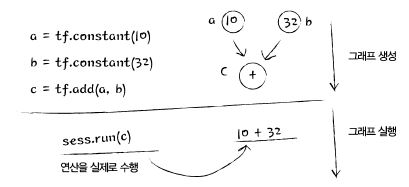
\includegraphics{./img/img1.JPG}
\caption{텐서플로 구조}
\end{figure}

\textbf{그래프}는 텐서들의 연산 모음이다.

텐서플로는 (1)텐서와 텐서의 연산들을 먼저 정의하여 그래프를 만들고 (2)
이후 필요할 때 연산을 실행하는 코드를 넣어 \emph{'원하는 시점'}에 실제
연산을 수행하도록 한다. 이러한 방식은 \textbf{지연 실행}이라하며 함수형
프로그래밍에서 많이 사용한다.

다음처럼 Session 객체와 run 메소드를 사용할 때 계산이 된다.

따라서 모델을 구성하는 것과, 실행하는 것을 분리하여 프로그램을 깔끔하게
작성할 수 있다.

    \begin{Verbatim}[commandchars=\\\{\}]
{\color{incolor}In [{\color{incolor}2}]:} \PY{c+c1}{\PYZsh{} 그래프를 실행할 세션을 구성한다.}
        \PY{n}{sess} \PY{o}{=} \PY{n}{tf}\PY{o}{.}\PY{n}{Session}\PY{p}{(}\PY{p}{)}
        
        \PY{c+c1}{\PYZsh{} sess.run : 설정한 텐서 그래프(변수나 수식)을 실행한다.}
        \PY{n+nb}{print}\PY{p}{(}\PY{n}{sess}\PY{o}{.}\PY{n}{run}\PY{p}{(}\PY{n}{hello}\PY{p}{)}\PY{p}{)}
        \PY{n+nb}{print}\PY{p}{(}\PY{n}{sess}\PY{o}{.}\PY{n}{run}\PY{p}{(}\PY{p}{[}\PY{n}{a}\PY{p}{,} \PY{n}{b}\PY{p}{,} \PY{n}{c}\PY{p}{]}\PY{p}{)}\PY{p}{)}
        
        \PY{c+c1}{\PYZsh{} 세션을 닫는다}
        \PY{n}{sess}\PY{o}{.}\PY{n}{close}\PY{p}{(}\PY{p}{)}
\end{Verbatim}


    \begin{Verbatim}[commandchars=\\\{\}]
b'Hello, TensorFlow!'
[10, 32, 42]

    \end{Verbatim}

    그래프의 실행은 Session안에서 이루어져야 하며, session객체와 run
메소드를 사용한다.

\paragraph{3.2 플레이스홀더와
변수}\label{uxd50cuxb808uxc774uxc2a4uxd640uxb354uxc640-uxbcc0uxc218}

\begin{itemize}
\tightlist
\item
  플레이스폴더
\end{itemize}

그래프에 사용할 입력값을 나중에 받기 위해 사용하는 매개변수

!. 변수는 그래프를 최적화하는 용도로 텐서플로가(학습함수들이) 학습한
결과를 갱신하기 위해 사용하는 변수이다.

    \begin{Verbatim}[commandchars=\\\{\}]
{\color{incolor}In [{\color{incolor}3}]:} \PY{c+c1}{\PYZsh{} None은 크기가 정해지지 않았음을 의미}
        \PY{n}{X} \PY{o}{=} \PY{n}{tf}\PY{o}{.}\PY{n}{placeholder}\PY{p}{(}\PY{n}{tf}\PY{o}{.}\PY{n}{float32}\PY{p}{,} \PY{p}{[}\PY{k+kc}{None}\PY{p}{,} \PY{l+m+mi}{3}\PY{p}{]}\PY{p}{)}
        \PY{n+nb}{print}\PY{p}{(}\PY{n}{X}\PY{p}{)}
\end{Verbatim}


    \begin{Verbatim}[commandchars=\\\{\}]
Tensor("Placeholder:0", shape=(?, 3), dtype=float32)

    \end{Verbatim}

    float32 자료형을 가진 텐서가 생성됐다.

나중에 플레이스홀더 X에 넣을 자료를 다음과 같이 정의해 볼 수 있다.

앞서 텐서 모양을 (?, 3)으로 정의했으므로, 두 번째 차원은 요소를 3개씩
가지고 있어야 한다.

    \begin{Verbatim}[commandchars=\\\{\}]
{\color{incolor}In [{\color{incolor}4}]:} \PY{n}{x\PYZus{}data} \PY{o}{=} \PY{p}{[}\PY{p}{[}\PY{l+m+mi}{1}\PY{p}{,}\PY{l+m+mi}{2}\PY{p}{,}\PY{l+m+mi}{3}\PY{p}{]}\PY{p}{,} \PY{p}{[}\PY{l+m+mi}{4}\PY{p}{,}\PY{l+m+mi}{5}\PY{p}{,}\PY{l+m+mi}{6}\PY{p}{]}\PY{p}{]}
        
        \PY{c+c1}{\PYZsh{}변수 정의}
        \PY{n}{W} \PY{o}{=} \PY{n}{tf}\PY{o}{.}\PY{n}{Variable}\PY{p}{(}\PY{n}{tf}\PY{o}{.}\PY{n}{random\PYZus{}normal}\PY{p}{(}\PY{p}{[}\PY{l+m+mi}{3}\PY{p}{,} \PY{l+m+mi}{2}\PY{p}{]}\PY{p}{)}\PY{p}{)}  \PY{c+c1}{\PYZsh{} random\PYZus{}normal : 정규분포의 무작위 값}
        \PY{n}{b} \PY{o}{=} \PY{n}{tf}\PY{o}{.}\PY{n}{Variable}\PY{p}{(}\PY{n}{tf}\PY{o}{.}\PY{n}{random\PYZus{}normal}\PY{p}{(}\PY{p}{[}\PY{l+m+mi}{2}\PY{p}{,} \PY{l+m+mi}{1}\PY{p}{]}\PY{p}{)}\PY{p}{)}
\end{Verbatim}


    각각 W와 b에 텐서플로 변수를 생성하여 할당한다.

W는 {[}3, 2{]} 행렬형태의 텐서, b는 {[}2, 1{]} 행렬 형대의 텐서로
정규분포의 무작위 값으로 초기화했다.

물론 다른 함수를 쓰거나 특정 형태의 데이터를 만들어서 넣어줄 수도 있다.

다음으로 입력값과 변수들을 계산할 수식을 작성한다.

X와 W가 행렬이기 때문에 marmul 함수를 사용해햐 한다.

\emph{행렬이 아닌 경우에는 단순히 곱셈 연산자나 mul함수를 사용}

    \begin{Verbatim}[commandchars=\\\{\}]
{\color{incolor}In [{\color{incolor}5}]:} \PY{n}{expr} \PY{o}{=} \PY{n}{tf}\PY{o}{.}\PY{n}{matmul}\PY{p}{(}\PY{n}{X}\PY{p}{,} \PY{n}{W}\PY{p}{)} \PY{o}{+} \PY{n}{b}
\end{Verbatim}


    \textbf{행렬곱 매우 중요}

\begin{figure}
\centering
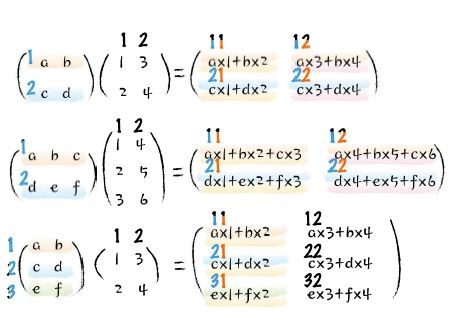
\includegraphics{./img/img2.JPG}
\caption{행렬곱}
\end{figure}

위 정의에 따라 앞서 X에 넣을 데이터를 {[}2,3{]} 형태로 정의하였으므로
행렬곱을 위해 W의 형태를 {[}3,2{]}로 정의한 것.

이제 연산을 실행하고 결과를 출력하여, 설정한 텐서들과 계산됭 그래프의
결과를 확인한다.

    \begin{Verbatim}[commandchars=\\\{\}]
{\color{incolor}In [{\color{incolor}6}]:} \PY{n}{sess} \PY{o}{=} \PY{n}{tf}\PY{o}{.}\PY{n}{Session}\PY{p}{(}\PY{p}{)}
        \PY{n}{sess}\PY{o}{.}\PY{n}{run}\PY{p}{(}\PY{n}{tf}\PY{o}{.}\PY{n}{global\PYZus{}variables\PYZus{}initializer}\PY{p}{(}\PY{p}{)}\PY{p}{)}   \PY{c+c1}{\PYZsh{} 앞서 정의한 변수들을 초기화하는 함수.}
        
        \PY{n+nb}{print}\PY{p}{(}\PY{l+s+s2}{\PYZdq{}}\PY{l+s+s2}{=== x\PYZus{}data ===}\PY{l+s+s2}{\PYZdq{}}\PY{p}{)}
        \PY{n+nb}{print}\PY{p}{(}\PY{n}{x\PYZus{}data}\PY{p}{)}
        \PY{n+nb}{print}\PY{p}{(}\PY{l+s+s2}{\PYZdq{}}\PY{l+s+s2}{=== W ===}\PY{l+s+s2}{\PYZdq{}}\PY{p}{)}
        \PY{n+nb}{print}\PY{p}{(}\PY{n}{sess}\PY{o}{.}\PY{n}{run}\PY{p}{(}\PY{n}{W}\PY{p}{)}\PY{p}{)}
        \PY{n+nb}{print}\PY{p}{(}\PY{l+s+s2}{\PYZdq{}}\PY{l+s+s2}{=== b ===}\PY{l+s+s2}{\PYZdq{}}\PY{p}{)}
        \PY{n+nb}{print}\PY{p}{(}\PY{n}{sess}\PY{o}{.}\PY{n}{run}\PY{p}{(}\PY{n}{b}\PY{p}{)}\PY{p}{)}
        \PY{n+nb}{print}\PY{p}{(}\PY{l+s+s2}{\PYZdq{}}\PY{l+s+s2}{=== expr ===}\PY{l+s+s2}{\PYZdq{}}\PY{p}{)}
        \PY{n+nb}{print}\PY{p}{(}\PY{n}{sess}\PY{o}{.}\PY{n}{run}\PY{p}{(}\PY{n}{expr}\PY{p}{,} \PY{n}{feed\PYZus{}dict}\PY{o}{=}\PY{p}{\PYZob{}}\PY{n}{X}\PY{p}{:} \PY{n}{x\PYZus{}data}\PY{p}{\PYZcb{}}\PY{p}{)}\PY{p}{)}    \PY{c+c1}{\PYZsh{} feed\PYZus{}dict : 그래프를 실행할 때 사용할 입력값을 지정한다.}
        
        \PY{n}{sess}\PY{o}{.}\PY{n}{close}\PY{p}{(}\PY{p}{)}
\end{Verbatim}


    \begin{Verbatim}[commandchars=\\\{\}]
=== x\_data ===
[[1, 2, 3], [4, 5, 6]]
=== W ===
[[-0.88866204 -0.09361325]
 [ 0.35012633  0.88960224]
 [ 0.550321   -0.6291377 ]]
=== b ===
[[ 2.053232]
 [-1.285216]]
=== expr ===
[[ 3.5157855   1.8514102 ]
 [ 0.21269333 -0.9864837 ]]

    \end{Verbatim}

    global\_variables\_initializer : 기존에 학습한 값을 가져와서 사용하는
것이 아닌 처음 실행하는 것이라면 연산을 실행하기 전에 반드시 이 함수를
이용해 변수들을 초기화해야 한다.

feed\_dict : expr 수식에는 X, W, b를 사용했는데, 이 중 X가
플레이스홀더라 X에 값을 넣어주지 않으면 계산에 사용할 수 없기 때문에
에러가 난다. 따라서 미리 정의해둔 x\_data를 X의 값으로 넣어준다.
\textbf{\emph{딕셔너리여도 되나??}}

\paragraph{3.3 선형 회귀 모델
구현}\label{uxc120uxd615-uxd68cuxadc0-uxbaa8uxb378-uxad6cuxd604}

\textbf{선형 회귀}란 주어진 x와 y값을 가지고 서로 간의 관계를 파악하는
것

이 관계를 알고나면 새로운 x가 주어졌을 때 y의 값을 쉽게 알 수 있다.

\begin{figure}
\centering
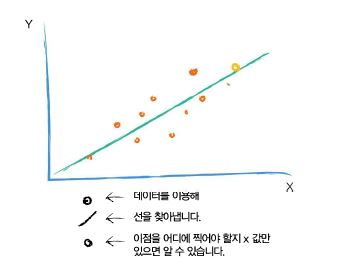
\includegraphics{./img/img3.JPG}
\caption{선형 회귀 그래프}
\end{figure}

이제 텐서플로의 최적화 함수를 이용해 X와 Y의 상관관계를 분석하는
기초적인 선형 회귀 모델을 만들고 실행해본다.

다음과 같이 주어진 x\_data와 y\_data의 상관관계를 파악해보자.

    \begin{Verbatim}[commandchars=\\\{\}]
{\color{incolor}In [{\color{incolor}7}]:} \PY{n}{x\PYZus{}data} \PY{o}{=} \PY{p}{[}\PY{l+m+mi}{1}\PY{p}{,} \PY{l+m+mi}{2}\PY{p}{,} \PY{l+m+mi}{3}\PY{p}{]}
        \PY{n}{y\PYZus{}data} \PY{o}{=} \PY{p}{[}\PY{l+m+mi}{1}\PY{p}{,} \PY{l+m+mi}{2}\PY{p}{,} \PY{l+m+mi}{3}\PY{p}{]}
        
        
        \PY{c+c1}{\PYZsh{} x와 y의 상관관계를 설명하기 위한 변수들인 W, b를 }
        \PY{c+c1}{\PYZsh{} 각각 \PYZhy{}0.1 \PYZti{} 1.0 사이의 균등분포를 가진 무작위값으로 초기화한다.}
        \PY{n}{W} \PY{o}{=} \PY{n}{tf}\PY{o}{.}\PY{n}{Variable}\PY{p}{(}\PY{n}{tf}\PY{o}{.}\PY{n}{random\PYZus{}uniform}\PY{p}{(}\PY{p}{[}\PY{l+m+mi}{1}\PY{p}{]}\PY{p}{,} \PY{o}{\PYZhy{}}\PY{l+m+mf}{1.0}\PY{p}{,} \PY{l+m+mf}{1.0}\PY{p}{)}\PY{p}{)}
        \PY{n}{b} \PY{o}{=} \PY{n}{tf}\PY{o}{.}\PY{n}{Variable}\PY{p}{(}\PY{n}{tf}\PY{o}{.}\PY{n}{random\PYZus{}uniform}\PY{p}{(}\PY{p}{[}\PY{l+m+mi}{1}\PY{p}{]}\PY{p}{,} \PY{o}{\PYZhy{}}\PY{l+m+mf}{1.0}\PY{p}{,} \PY{l+m+mf}{1.0}\PY{p}{)}\PY{p}{)}
        
        \PY{c+c1}{\PYZsh{} 자료를 입력받을 플레이스홀더 설정}
        \PY{c+c1}{\PYZsh{} name: 나중에 텐서보드등으로 값의 변화를 추적하거나 살펴보기 쉽게 하기 위해 이름을 붙여줍니다.}
        \PY{n}{X} \PY{o}{=} \PY{n}{tf}\PY{o}{.}\PY{n}{placeholder}\PY{p}{(}\PY{n}{tf}\PY{o}{.}\PY{n}{float32}\PY{p}{,} \PY{n}{name}\PY{o}{=}\PY{l+s+s2}{\PYZdq{}}\PY{l+s+s2}{X}\PY{l+s+s2}{\PYZdq{}}\PY{p}{)}
        \PY{n}{Y} \PY{o}{=} \PY{n}{tf}\PY{o}{.}\PY{n}{placeholder}\PY{p}{(}\PY{n}{tf}\PY{o}{.}\PY{n}{float32}\PY{p}{,} \PY{n}{name}\PY{o}{=}\PY{l+s+s2}{\PYZdq{}}\PY{l+s+s2}{Y}\PY{l+s+s2}{\PYZdq{}}\PY{p}{)}
        
        \PY{c+c1}{\PYZsh{} X와 Y의 상관관계(여기서는 선형관계)를 분석하기 위한 수실을 작성한다.}
        \PY{n}{hypothesis} \PY{o}{=} \PY{n}{W} \PY{o}{*} \PY{n}{X} \PY{o}{+} \PY{n}{b}    
\end{Verbatim}


    위 수식은 W와의 곱과 b와의 합을 통해 X와 Y의 관계를 설명하겠다는 뜻이다.

\textbf{다시말해서 X가 주어졌을 때 Y를 만들어 낼 수 있는 W와 b를
찾아내겠다는 의미.}

W는 \textbf{가중치}, b는 \textbf{편향}이라고 하고, 위 수식은 신경망
학습에서 가장 기본이 되는 수식이다. 여기서는 w와 X가 행렬이 아니므로
tf.matmul 함수가 아니라 곱셈 연산자(*)를 사용했다.

    \begin{Verbatim}[commandchars=\\\{\}]
{\color{incolor}In [{\color{incolor}8}]:} \PY{c+c1}{\PYZsh{} 손실 함수를 작성한다.}
        \PY{c+c1}{\PYZsh{} mean(h \PYZhy{} Y)\PYZca{}2 : 예측값과 실제값의 거리를 비용(손실) 함수로 정합니다.}
        \PY{n}{cost} \PY{o}{=} \PY{n}{tf}\PY{o}{.}\PY{n}{reduce\PYZus{}mean}\PY{p}{(}\PY{n}{tf}\PY{o}{.}\PY{n}{square}\PY{p}{(}\PY{n}{hypothesis} \PY{o}{\PYZhy{}} \PY{n}{Y}\PY{p}{)}\PY{p}{)}
\end{Verbatim}


    \textbf{손실 함수(loss function)}는 한 쌍(x,y)의 데이터에 대한 손실값을
계산하는 함수이다.

손실값이란 실제값과 모델로 예측한 가설의 값이 얼마나 차이가 나는가를
나타내는 값이다.

즉, 손실값이 작을수록 그 모델이 X와 Y의 관계를 잘 설명하고 있는다는
뜻으로 \emph{X값에 대한 Y값을 정확하게 예측할 수 있다}는 뜻이 된다.

이 손실을 전체 데이터에 대해 구한 경우 이를 \textbf{비용}이라고 한다.

즉, \textbf{학습}이란 변수들의 값을 다양하게 넣어 계산해보면서 이
\textbf{손실값을 최소화하는 W와 b의 값을 구하는 것}이다.

손실값으로는 '예측값과 실제값의 거리'를 가장 많이 사용한다.

손실값은 예측값에서 실제값을 뺀 뒤 제곱하는데, 비용은 모든 데이터에 대한
손실값의 평균을 내어 구한다.

마지막으로 경사하강법 최적화 함수를 이용해 손실값을 최소화하는 연산
그래프를 생성한다.

    \begin{Verbatim}[commandchars=\\\{\}]
{\color{incolor}In [{\color{incolor}9}]:} \PY{c+c1}{\PYZsh{} 경사하강법 최적화 함수를 이용해 손실값을 최소화하는 연산 그래프 생성}
        \PY{n}{optimizer} \PY{o}{=} \PY{n}{tf}\PY{o}{.}\PY{n}{train}\PY{o}{.}\PY{n}{GradientDescentOptimizer}\PY{p}{(}\PY{n}{learning\PYZus{}rate}\PY{o}{=}\PY{l+m+mf}{0.1}\PY{p}{)}
        \PY{n}{train\PYZus{}op} \PY{o}{=} \PY{n}{optimizer}\PY{o}{.}\PY{n}{minimize}\PY{p}{(}\PY{n}{cost}\PY{p}{)}
\end{Verbatim}


    \textbf{최적화함수}란 가중치와 편향의 값을 변경해가면서 손실값을
최소화하는 \emph{가장 최적화된 가중치와 편향 값을 찾아주는 함수}이다.

이때 값들을 무작위로 변경하면 시간이 오래걸리고 예측도 쉽지 않다. 따라서
빠르게 최적화하기 위한 다양한 방법을 사용한다.

경사하강법은 최적화 방법 중 가장 기본적인 알고리즘으로,

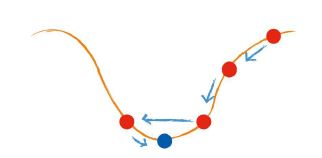
\includegraphics{./img/img4.JPG} 함수의 기울기를 구하고 기울기가 낮은
족으로 계속 이동시키면서 최적의 값을 찾아가는 방법이다.

매개변수인 learning\_rate는 \textbf{학습률}로 학습을 얼마나 "급하게"할
것인가를 설정하는 값이다. 값이 너무 크거나 작으면 좋지 않다. (크면
최적의 값을 찾지 못하고, 작으면 속도가 느리다)

이렇게 학습 진행 과정에 영향을 주는 변수를 \textbf{하이퍼파라미터}라고
하며, 이 값에 따라 속도나 성능이 크게 달라질 수 있다.

이제 모델은 다 만들었고, 그래프를 실행해 학습시키고 결과를 확인한다.

    \begin{Verbatim}[commandchars=\\\{\}]
{\color{incolor}In [{\color{incolor}17}]:} \PY{c+c1}{\PYZsh{} 세션은 생성하고 변수들을 초기화 한다. }
         \PY{c+c1}{\PYZsh{} 파이썬 with 기능을 이용해 세션 블록을 만들고 종료를 자동으로 처리하도록 했다.}
         \PY{k}{with} \PY{n}{tf}\PY{o}{.}\PY{n}{Session}\PY{p}{(}\PY{p}{)} \PY{k}{as} \PY{n}{sess}\PY{p}{:}
             \PY{n}{sess}\PY{o}{.}\PY{n}{run}\PY{p}{(}\PY{n}{tf}\PY{o}{.}\PY{n}{global\PYZus{}variables\PYZus{}initializer}\PY{p}{(}\PY{p}{)}\PY{p}{)}
         
             \PY{c+c1}{\PYZsh{} 최적화를 수행하는 그래프인 train\PYZus{}op를 실행하고}
             \PY{c+c1}{\PYZsh{} 실행 시마다 변화하는 손실값을 출력하는 코드}
             \PY{c+c1}{\PYZsh{} 학습은 100번 수행하며 feed\PYZus{}dict 매개변수로 상관관계를 알아내고자 하는 x\PYZus{}data, y\PYZus{}data를 입력해준다.}
             \PY{k}{for} \PY{n}{step} \PY{o+ow}{in} \PY{n+nb}{range}\PY{p}{(}\PY{l+m+mi}{100}\PY{p}{)}\PY{p}{:}
                 \PY{n}{\PYZus{}}\PY{p}{,} \PY{n}{cost\PYZus{}val} \PY{o}{=} \PY{n}{sess}\PY{o}{.}\PY{n}{run}\PY{p}{(}\PY{p}{[}\PY{n}{train\PYZus{}op}\PY{p}{,} \PY{n}{cost}\PY{p}{]}\PY{p}{,} \PY{n}{feed\PYZus{}dict}\PY{o}{=}\PY{p}{\PYZob{}}\PY{n}{X}\PY{p}{:} \PY{n}{x\PYZus{}data}\PY{p}{,} \PY{n}{Y}\PY{p}{:} \PY{n}{y\PYZus{}data}\PY{p}{\PYZcb{}}\PY{p}{)}
         
                 \PY{n+nb}{print}\PY{p}{(}\PY{n}{step}\PY{p}{,} \PY{n}{cost\PYZus{}val}\PY{p}{,} \PY{n}{sess}\PY{o}{.}\PY{n}{run}\PY{p}{(}\PY{n}{W}\PY{p}{)}\PY{p}{,} \PY{n}{sess}\PY{o}{.}\PY{n}{run}\PY{p}{(}\PY{n}{b}\PY{p}{)}\PY{p}{)}
                 
             \PY{c+c1}{\PYZsh{} 최적화가 완료된 모델에 테스트 값을 넣고 결과가 나오는지 확인}
             \PY{n+nb}{print}\PY{p}{(}\PY{l+s+s2}{\PYZdq{}}\PY{l+s+se}{\PYZbs{}n}\PY{l+s+s2}{=====Test=========}\PY{l+s+s2}{\PYZdq{}}\PY{p}{)}
             \PY{n+nb}{print}\PY{p}{(}\PY{l+s+s2}{\PYZdq{}}\PY{l+s+s2}{X: 5, Y:}\PY{l+s+s2}{\PYZdq{}}\PY{p}{,} \PY{n}{sess}\PY{o}{.}\PY{n}{run}\PY{p}{(}\PY{n}{hypothesis}\PY{p}{,} \PY{n}{feed\PYZus{}dict}\PY{o}{=}\PY{p}{\PYZob{}}\PY{n}{X}\PY{p}{:} \PY{l+m+mi}{5}\PY{p}{\PYZcb{}}\PY{p}{)}\PY{p}{)}
             \PY{n+nb}{print}\PY{p}{(}\PY{l+s+s2}{\PYZdq{}}\PY{l+s+s2}{X: 2.5, Y:}\PY{l+s+s2}{\PYZdq{}}\PY{p}{,} \PY{n}{sess}\PY{o}{.}\PY{n}{run}\PY{p}{(}\PY{n}{hypothesis}\PY{p}{,} \PY{n}{feed\PYZus{}dict}\PY{o}{=}\PY{p}{\PYZob{}}\PY{n}{X}\PY{p}{:} \PY{l+m+mf}{2.5}\PY{p}{\PYZcb{}}\PY{p}{)}\PY{p}{)}
\end{Verbatim}


    \begin{Verbatim}[commandchars=\\\{\}]
0 0.27773085 [0.5816037] [0.9928714]
1 0.14106424 [0.5749584] [0.9616557]
2 0.13288867 [0.5870016] [0.9393412]
3 0.12655877 [0.5967303] [0.9166723]
4 0.1205469 [0.60644644] [0.8946457]
5 0.11482086 [0.6159048] [0.87313795]
6 0.10936674 [0.62513846] [0.8521484]
7 0.1041717 [0.63414985] [0.83166337]
8 0.09922349 [0.64294463] [0.8116707]
9 0.09451029 [0.651528] [0.7921587]
10 0.090021014 [0.659905] [0.77311575]
11 0.08574492 [0.6680807] [0.7545306]
12 0.08167198 [0.6760598] [0.7363922]
13 0.07779249 [0.68384707] [0.71868986]
14 0.07409727 [0.69144714] [0.70141304]
15 0.07057763 [0.6988646] [0.6845516]
16 0.067225106 [0.7061036] [0.6680954]
17 0.06403191 [0.71316874] [0.6520349]
18 0.060990345 [0.7200639] [0.6363604]
19 0.058093254 [0.7267934] [0.62106276]
20 0.055333775 [0.7333611] [0.6061328]
21 0.05270542 [0.739771] [0.5915618]
22 0.050201822 [0.74602664] [0.577341]
23 0.047817186 [0.752132] [0.56346214]
24 0.04554588 [0.7580906] [0.5499169]
25 0.043382373 [0.7639059] [0.53669727]
26 0.0413217 [0.7695815] [0.5237955]
27 0.039358873 [0.77512056] [0.51120377]
28 0.03748929 [0.7805265] [0.4989148]
29 0.035708573 [0.78580254] [0.48692125]
30 0.034012362 [0.79095167] [0.47521597]
31 0.032396767 [0.79597706] [0.46379212]
32 0.0308579 [0.8008816] [0.45264286]
33 0.029392116 [0.8056683] [0.4417616]
34 0.027995946 [0.8103399] [0.43114197]
35 0.026666136 [0.81489927] [0.42077762]
36 0.02539947 [0.8193489] [0.41066238]
37 0.024192961 [0.8236916] [0.40079036]
38 0.023043783 [0.8279299] [0.39115563]
39 0.021949196 [0.8320664] [0.38175255]
40 0.020906614 [0.83610344] [0.3725755]
41 0.019913519 [0.84004337] [0.363619]
42 0.018967599 [0.8438886] [0.35487783]
43 0.018066624 [0.8476414] [0.34634683]
44 0.01720845 [0.85130405] [0.33802092]
45 0.016391046 [0.8548786] [0.32989514]
46 0.01561246 [0.8583672] [0.32196468]
47 0.014870856 [0.86177194] [0.31422484]
48 0.0141644925 [0.8650949] [0.3066711]
49 0.013491653 [0.86833787] [0.2992989]
50 0.01285078 [0.87150294] [0.29210398]
51 0.012240354 [0.87459195] [0.285082]
52 0.011658926 [0.87760663] [0.27822882]
53 0.011105127 [0.88054895] [0.2715404]
54 0.010577627 [0.8834204] [0.26501274]
55 0.010075196 [0.8862229] [0.25864202]
56 0.009596606 [0.88895804] [0.25242445]
57 0.009140749 [0.89162743] [0.24635635]
58 0.008706565 [0.89423263] [0.24043411]
59 0.008292996 [0.8967752] [0.23465423]
60 0.007899082 [0.89925665] [0.22901331]
61 0.007523867 [0.9016785] [0.223508]
62 0.0071664653 [0.904042] [0.218135]
63 0.006826054 [0.90634876] [0.21289119]
64 0.006501818 [0.9086001] [0.20777345]
65 0.006192978 [0.9107973] [0.20277873]
66 0.005898807 [0.91294163] [0.19790407]
67 0.005618608 [0.9150345] [0.1931466]
68 0.0053517236 [0.917077] [0.18850349]
69 0.005097508 [0.9190704] [0.183972]
70 0.004855378 [0.9210159] [0.17954944]
71 0.004624739 [0.9229146] [0.1752332]
72 0.004405064 [0.9247677] [0.17102072]
73 0.004195818 [0.92657626] [0.16690952]
74 0.003996516 [0.92834127] [0.16289711]
75 0.0038066825 [0.9300639] [0.15898119]
76 0.0036258616 [0.9317452] [0.1551594]
77 0.003453619 [0.93338585] [0.15142943]
78 0.0032895773 [0.9349873] [0.14778921]
79 0.0031333212 [0.93655014] [0.14423645]
80 0.0029844828 [0.93807536] [0.14076908]
81 0.0028427206 [0.93956405] [0.13738512]
82 0.0027076832 [0.9410169] [0.13408248]
83 0.002579068 [0.9424348] [0.13085921]
84 0.0024565673 [0.9438186] [0.12771346]
85 0.0023398772 [0.94516915] [0.1246433]
86 0.002228728 [0.9464873] [0.12164699]
87 0.002122869 [0.94777375] [0.11872269]
88 0.0020220275 [0.94902915] [0.11586864]
89 0.0019259813 [0.9502545] [0.11308326]
90 0.0018344905 [0.9514503] [0.11036479]
91 0.0017473547 [0.95261747] [0.10771173]
92 0.0016643492 [0.95375645] [0.10512239]
93 0.0015852948 [0.95486814] [0.10259533]
94 0.0015099873 [0.95595306] [0.10012902]
95 0.0014382672 [0.95701194] [0.09772198]
96 0.0013699448 [0.9580453] [0.0953728]
97 0.0013048725 [0.9590539] [0.0930801]
98 0.0012428967 [0.96003824] [0.09084255]
99 0.0011838536 [0.96099883] [0.08865874]

=====Test=========
X: 5, Y: [4.893653]
X: 2.5, Y: [2.4911559]

    \end{Verbatim}

    손실값과 변수들의 변화를 확인 할 수 있다.

손실값이 점점 줄어든다면 학습이 정상적으로 이뤄지고있는 것이다.

*** \_ 는 뭐지


    % Add a bibliography block to the postdoc
    
    
    
    \end{document}
